%===============================================================================
% LaTeX sjabloon voor de bachelorproef toegepaste informatica aan HOGENT
% Meer info op https://github.com/HoGentTIN/latex-hogent-report
%===============================================================================

\documentclass[dutch,dit,thesis]{hogentreport}

% TODO:
% - If necessary, replace the option `dit`' with your own department!
%   Valid entries are dbo, dbt, dgz, dit, dlo, dog, dsa, soa
% - If you write your thesis in English (remark: only possible after getting
%   explicit approval!), remove the option "dutch," or replace with "english".

\usepackage{lipsum} % For blind text, can be removed after adding actual content

%% Pictures to include in the text can be put in the graphics/ folder
\graphicspath{{graphics/}}

%% For source code highlighting, requires pygments to be installed
%% Compile with the -shell-escape flag!
\usepackage[section]{minted}
%% If you compile with the make_thesis.{bat,sh} script, use the following
%% import instead:
%% \usepackage[section,outputdir=../output]{minted}
\usemintedstyle{solarized-light}
\definecolor{bg}{RGB}{253,246,227} %% Set the background color of the codeframe

%% Change this line to edit the line numbering style:
\renewcommand{\theFancyVerbLine}{\ttfamily\scriptsize\arabic{FancyVerbLine}}

%% Macro definition to load external java source files with \javacode{filename}:
\newmintedfile[javacode]{java}{
    bgcolor=bg,
    fontfamily=tt,
    linenos=true,
    numberblanklines=true,
    numbersep=5pt,
    gobble=0,
    framesep=2mm,
    funcnamehighlighting=true,
    tabsize=4,
    obeytabs=false,
    breaklines=true,
    mathescape=false
    samepage=false,
    showspaces=false,
    showtabs =false,
    texcl=false,
}

% Other packages not already included can be imported here

%%---------- Document metadata -------------------------------------------------
% TODO: Replace this with your own information
\author{Anasio Claeys}
\supervisor{Dhr. P. Van Der Helst}
\cosupervisor{Dhr. G. Vercammen}
\title[]%
    {Het integreren van spraakherkenningstechnologie op apparaten met beperkte middelen: vergelijkende studie en\\ proof-of-concept.}
\academicyear{\advance\year by -1 \the\year--\advance\year by 1 \the\year}
\examperiod{1}
\degreesought{\IfLanguageName{dutch}{Professionele bachelor in de toegepaste informatica}{Bachelor of applied computer science}}
\partialthesis{false} %% To display 'in partial fulfilment'
%\institution{Internshipcompany BVBA.}

%% Add global exceptions to the hyphenation here
\hyphenation{back-slash}

%% The bibliography (style and settings are  found in hogentthesis.cls)
\addbibresource{bachproef.bib}            %% Bibliography file
\addbibresource{../voorstel/voorstel.bib} %% Bibliography research proposal
\defbibheading{bibempty}{}

%% Prevent empty pages for right-handed chapter starts in twoside mode
\renewcommand{\cleardoublepage}{\clearpage}

\renewcommand{\arraystretch}{1.2}

%% Content starts here.
\begin{document}

%---------- Front matter -------------------------------------------------------

\frontmatter

\hypersetup{pageanchor=false} %% Disable page numbering references
%% Render a Dutch outer title page if the main language is English
\IfLanguageName{english}{%
    %% If necessary, information can be changed here
    \degreesought{Professionele Bachelor toegepaste informatica}%
    \begin{otherlanguage}{dutch}%
       \maketitle%
    \end{otherlanguage}%
}{}

%% Generates title page content
\maketitle
\hypersetup{pageanchor=true}

%%=============================================================================
%% Voorwoord
%%=============================================================================

\chapter*{\IfLanguageName{dutch}{Woord vooraf}{Preface}}%
\label{ch:voorwoord}

%% TODO:
%% Het voorwoord is het enige deel van de bachelorproef waar je vanuit je
%% eigen standpunt (``ik-vorm'') mag schrijven. Je kan hier bv. motiveren
%% waarom jij het onderwerp wil bespreken.
%% Vergeet ook niet te bedanken wie je geholpen/gesteund/... heeft

\lipsum[1-2]
%%=============================================================================
%% Samenvatting
%%=============================================================================

% TODO: De "abstract" of samenvatting is een kernachtige (~ 1 blz. voor een
% thesis) synthese van het document.
%
% Een goede abstract biedt een kernachtig antwoord op volgende vragen:
%
% 1. Waarover gaat de bachelorproef?
% 2. Waarom heb je er over geschreven?
% 3. Hoe heb je het onderzoek uitgevoerd?
% 4. Wat waren de resultaten? Wat blijkt uit je onderzoek?
% 5. Wat betekenen je resultaten? Wat is de relevantie voor het werkveld?
%
% Daarom bestaat een abstract uit volgende componenten:
%
% - inleiding + kaderen thema
% - probleemstelling
% - (centrale) onderzoeksvraag
% - onderzoeksdoelstelling
% - methodologie
% - resultaten (beperk tot de belangrijkste, relevant voor de onderzoeksvraag)
% - conclusies, aanbevelingen, beperkingen
%
% LET OP! Een samenvatting is GEEN voorwoord!

%%---------- Nederlandse samenvatting -----------------------------------------
%
% TODO: Als je je bachelorproef in het Engels schrijft, moet je eerst een
% Nederlandse samenvatting invoegen. Haal daarvoor onderstaande code uit
% commentaar.
% Wie zijn bachelorproef in het Nederlands schrijft, kan dit negeren, de inhoud
% wordt niet in het document ingevoegd.

\IfLanguageName{english}{%
\selectlanguage{dutch}
\chapter*{Samenvatting}
\lipsum[1-4]
\selectlanguage{english}
}{}

%%---------- Samenvatting -----------------------------------------------------
% De samenvatting in de hoofdtaal van het document

\chapter*{\IfLanguageName{dutch}{Samenvatting}{Abstract}}

% \lipsum[1-4]
TO DO


%---------- Inhoud, lijst figuren, ... -----------------------------------------

\tableofcontents

% In a list of figures, the complete caption will be included. To prevent this,
% ALWAYS add a short description in the caption!
%
%  \caption[short description]{elaborate description}
%
% If you do, only the short description will be used in the list of figures

\listoffigures

% If you included tables and/or source code listings, uncomment the appropriate
% lines.
%\listoftables
%\listoflistings

% Als je een lijst van afkortingen of termen wil toevoegen, dan hoort die
% hier thuis. Gebruik bijvoorbeeld de ``glossaries'' package.
% https://www.overleaf.com/learn/latex/Glossaries

%---------- Kern ---------------------------------------------------------------

\mainmatter{}

% De eerste hoofdstukken van een bachelorproef zijn meestal een inleiding op
% het onderwerp, literatuurstudie en verantwoording methodologie.
% Aarzel niet om een meer beschrijvende titel aan deze hoofdstukken te geven of
% om bijvoorbeeld de inleiding en/of stand van zaken over meerdere hoofdstukken
% te verspreiden!

%%=============================================================================
%% Inleiding
%%=============================================================================

\chapter{\IfLanguageName{dutch}{Inleiding}{Introduction}}%
\label{ch:inleiding}

De inleiding moet de lezer net genoeg informatie verschaffen om het onderwerp te begrijpen en in te zien waarom de onderzoeksvraag de moeite waard is om te onderzoeken. In de inleiding ga je literatuurverwijzingen beperken, zodat de tekst vlot leesbaar blijft. Je kan de inleiding verder onderverdelen in secties als dit de tekst verduidelijkt. Zaken die aan bod kunnen komen in de inleiding~\autocite{Pollefliet2011}:

\begin{itemize}
  \item context, achtergrond
  \item afbakenen van het onderwerp
  \item verantwoording van het onderwerp, methodologie
  \item probleemstelling
  \item onderzoeksdoelstelling
  \item onderzoeksvraag
  \item \ldots
\end{itemize}

\section{\IfLanguageName{dutch}{Probleemstelling}{Problem Statement}}%
\label{sec:probleemstelling}

Uit je probleemstelling moet duidelijk zijn dat je onderzoek een meerwaarde heeft voor een concrete doelgroep. De doelgroep moet goed gedefinieerd en afgelijnd zijn. Doelgroepen als ``bedrijven,'' ``KMO's'', systeembeheerders, enz.~zijn nog te vaag. Als je een lijstje kan maken van de personen/organisaties die een meerwaarde zullen vinden in deze bachelorproef (dit is eigenlijk je steekproefkader), dan is dat een indicatie dat de doelgroep goed gedefinieerd is. Dit kan een enkel bedrijf zijn of zelfs één persoon (je co-promotor/opdrachtgever).

\section{\IfLanguageName{dutch}{Onderzoeksvraag}{Research question}}%
\label{sec:onderzoeksvraag}

Wees zo concreet mogelijk bij het formuleren van je onderzoeksvraag. Een onderzoeksvraag is trouwens iets waar nog niemand op dit moment een antwoord heeft (voor zover je kan nagaan). Het opzoeken van bestaande informatie (bv. ``welke tools bestaan er voor deze toepassing?'') is dus geen onderzoeksvraag. Je kan de onderzoeksvraag verder specifiëren in deelvragen. Bv.~als je onderzoek gaat over performantiemetingen, dan 

\section{\IfLanguageName{dutch}{Onderzoeksdoelstelling}{Research objective}}%
\label{sec:onderzoeksdoelstelling}

Wat is het beoogde resultaat van je bachelorproef? Wat zijn de criteria voor succes? Beschrijf die zo concreet mogelijk. Gaat het bv.\ om een proof-of-concept, een prototype, een verslag met aanbevelingen, een vergelijkende studie, enz.

\section{\IfLanguageName{dutch}{Opzet van deze bachelorproef}{Structure of this bachelor thesis}}%
\label{sec:opzet-bachelorproef}

% Het is gebruikelijk aan het einde van de inleiding een overzicht te
% geven van de opbouw van de rest van de tekst. Deze sectie bevat al een aanzet
% die je kan aanvullen/aanpassen in functie van je eigen tekst.

De rest van deze bachelorproef is als volgt opgebouwd:

In Hoofdstuk~\ref{ch:stand-van-zaken} wordt een overzicht gegeven van de stand van zaken binnen het onderzoeksdomein, op basis van een literatuurstudie.

In Hoofdstuk~\ref{ch:methodologie} wordt de methodologie toegelicht en worden de gebruikte onderzoekstechnieken besproken om een antwoord te kunnen formuleren op de onderzoeksvragen.

% TODO: Vul hier aan voor je eigen hoofstukken, één of twee zinnen per hoofdstuk

In Hoofdstuk~\ref{ch:conclusie}, tenslotte, wordt de conclusie gegeven en een antwoord geformuleerd op de onderzoeksvragen. Daarbij wordt ook een aanzet gegeven voor toekomstig onderzoek binnen dit domein.
\chapter{\IfLanguageName{dutch}{Stand van zaken}{State of the art}}%
\label{ch:stand-van-zaken}

% Tip: Begin elk hoofdstuk met een paragraaf inleiding die beschrijft hoe
% dit hoofdstuk past binnen het geheel van de bachelorproef. Geef in het
% bijzonder aan wat de link is met het vorige en volgende hoofdstuk.

% Pas na deze inleidende paragraaf komt de eerste sectiehoofding.

Dit hoofdstuk bevat je literatuurstudie. De inhoud gaat verder op de inleiding, maar zal het onderwerp van de bachelorproef *diepgaand* uitspitten. De bedoeling is dat de lezer na lezing van dit hoofdstuk helemaal op de hoogte is van de huidige stand van zaken (state-of-the-art) in het onderzoeksdomein. Iemand die niet vertrouwd is met het onderwerp, weet nu voldoende om de rest van het verhaal te kunnen volgen, zonder dat die er nog andere informatie moet over opzoeken \autocite{Pollefliet2011}.

Je verwijst bij elke bewering die je doet, vakterm die je introduceert, enz.\ naar je bronnen. In \LaTeX{} kan dat met het commando \texttt{$\backslash${textcite\{\}}} of \texttt{$\backslash${autocite\{\}}}. Als argument van het commando geef je de ``sleutel'' van een ``record'' in een bibliografische databank in het Bib\LaTeX{}-formaat (een tekstbestand). Als je expliciet naar de auteur verwijst in de zin (narratieve referentie), gebruik je \texttt{$\backslash${}textcite\{\}}. Soms is de auteursnaam niet expliciet een onderdeel van de zin, dan gebruik je \texttt{$\backslash${}autocite\{\}} (referentie tussen haakjes). Dit gebruik je bv.~bij een citaat, of om in het bijschrift van een overgenomen afbeelding, broncode, tabel, enz. te verwijzen naar de bron. In de volgende paragraaf een voorbeeld van elk.

\textcite{Knuth1998} schreef een van de standaardwerken over sorteer- en zoekalgoritmen. Experten zijn het erover eens dat cloud computing een interessante opportuniteit vormen, zowel voor gebruikers als voor dienstverleners op vlak van informatietechnologie~\autocite{Creeger2009}.

Let er ook op: het \texttt{cite}-commando voor de punt, dus binnen de zin. Je verwijst meteen naar een bron in de eerste zin die erop gebaseerd is, dus niet pas op het einde van een paragraaf.

\lipsum[7-20]

%%=============================================================================
%% Methodologie
%%=============================================================================

\chapter{\IfLanguageName{dutch}{Methodologie}{Methodology}}%
\label{ch:methodologie}

%% TODO: In dit hoofstuk geef je een korte toelichting over hoe je te werk bent
%% gegaan. Verdeel je onderzoek in grote fasen, en licht in elke fase toe wat
%% de doelstelling was, welke deliverables daar uit gekomen zijn, en welke
%% onderzoeksmethoden je daarbij toegepast hebt. Verantwoord waarom je
%% op deze manier te werk gegaan bent.
%% 
%% Voorbeelden van zulke fasen zijn: literatuurstudie, opstellen van een
%% requirements-analyse, opstellen long-list (bij vergelijkende studie),
%% selectie van geschikte tools (bij vergelijkende studie, "short-list"),
%% opzetten testopstelling/PoC, uitvoeren testen en verzamelen
%% van resultaten, analyse van resultaten, ...
%%
%% !!!!! LET OP !!!!!
%%
%% Het is uitdrukkelijk NIET de bedoeling dat je het grootste deel van de corpus
%% van je bachelorproef in dit hoofstuk verwerkt! Dit hoofdstuk is eerder een
%% kort overzicht van je plan van aanpak.
%%
%% Maak voor elke fase (behalve het literatuuronderzoek) een NIEUW HOOFDSTUK aan
%% en geef het een gepaste titel.

\lipsum[21-25]



% Voeg hier je eigen hoofdstukken toe die de ``corpus'' van je bachelorproef
% vormen. De structuur en titels hangen af van je eigen onderzoek. Je kan bv.
% elke fase in je onderzoek in een apart hoofdstuk bespreken.

%\input{...}
%\input{...}
%...
%%=============================================================================
%% Selectie van spraakmodellen
%% Long list & Short list
%%=============================================================================

\chapter{\IfLanguageName{dutch}{Selectie van spraakmodellen}{Selectie van spraakmodellen}}%
\label{ch:Selectie van spraakmodellen}

Nadat we een beter inzicht hebben verkregen in de verschillende fases van het onderzoek en de requirements hebben vastgelegd, is het tijd om de spraakmodellen te selecteren die zullen worden vergeleken. In dit hoofdstuk wordt er eerst een long list opgesteld van spraakmodellen die voldoen aan de vastgelegde requirements. Op basis van deze long list zullen we vervolgens een short list opstellen van de meest geschikte spraakmodellen.

\section{Long list}
In die long list zullen de spraakmodellen opgesomd worden die voldoen aan de vastgelegde requirements. Het MoSCoW-principe zal hierbij als leidraad dienen. De long list zal bestaan uit spraakmodellen die voldoen aan de meeste voorwaarden van de ``Must have`` en ``Should have`` requirements.

\begin{itemize}
  \item Google Cloud Speech-to-Text
  \item Microsoft Azure Speech-to-Text (Embedded)
  \item Mozilla DeepSpeech
  \item Kaldi
  \item PocketSphinx
  \item Vosk
  \item Whisper
  \item PicoVoice Cheetah
  \item IBM Watson Speech to Text
  \item Amazon Transcribe
  \item Baidu DeepSpeech
\end{itemize}

\section{Short list}
Na de long list is het tijd om een short list op te stellen van de meest geschikte spraakmodellen. Dit zal gebeuren in samenspraak met delaware.

\begin{itemize}
  \item Vosk
  \item Microsoft Azure Speech-to-Text (Embedded)
  \item Mozilla DeepSpeech
  \item Whisper
  \item PicoVoice Cheetah
\end{itemize}

%%=============================================================================
%% Selectie van spraakdata
%%=============================================================================

\chapter{\IfLanguageName{dutch}{Selectie van spraakdata}{Selectie van spraakdata}}%
\label{ch:Selectie van spraakdata}

Nu de spraakmodellen geselecteerd zijn, is het tijd om de spraakdata te selecteren die gebruikt zullen worden om deze modellen te vergelijken. In dit hoofdstuk zullen de verschillende stappen worden toegelicht om de spraakdata te selecteren. Het is heel belangrijk dat er voldoende spraakdata worden geselecteerd die representatief zijn en een duidelijk beeld geven van de prestaties van de spraakmodellen. Er worden drie talen getest, namelijk Engels, Frans en Nederlands. Voor elk van deze talen zullen er verschillende soorten spraakdata worden verzameld, waaronder verschillende accenten en dialecten. Het is de bedoeling dat de spraakdata zowel luide als stille omgevingsgeluiden bevatten zodat de spraakmodellen in beide omstandigheden kunnen worden getest. Op deze manier kan men de accuraatheid van de spraakmodellen evalueren en vergelijken via de Word Error Rate (WER). Het is dus van groot belang dat de spraakdata zorgvuldig worden geselecteerd. Bij de selectie van de spraakdata is het ook heel belangrijk dat de spraakdata voldoet aan de gebruikersrechten en privacywetgeving. Wat betreft de privacywetgeving is het belangrijk dat de spraakdata anoniem is en dat er geen persoonlijke gegevens worden opgeslagen. Bij de spraakdata moet er ook een geschreven transcriptie aanwezig zijn zodat de resultaten van de spraakmodellen kunnen worden geëvalueerd.

%%=============================================================================
%% Vergelijkende studie
%%=============================================================================

\chapter{\IfLanguageName{dutch}{Vergelijkende studie}{Vergelijkende studie}}%
\label{ch:Vergelijkende studie}

In dit hoofdstuk zullen we de spraakmodellen die geselecteerd zijn in de short list vergelijken met elkaar. Deze worden geïmplementeerd op de nieuwste versie van het besturingssysteem Android. We evalueren deze modellen op basis van diverse criteria, waaronder:

\begin{itemize}
  \item Documentatie
  \item Implementatie
  \item Performantie
  \item Accuraatheid
  \item Taalondersteuning
  \item Kostprijs
\end{itemize}

Deze vergelijking zal ons in staat stellen de sterktes en zwaktes van elk model te identificeren en zo het meest geschikte spraakmodel voor het onderzoek te selecteren.

\section{Vosk}
Vosk is een open-source spraakherkenningstechnologie die een toolkit aanbiedt voor het ontwikkelen van spraakherkenning in applicaties. Het maakt gebruik van algoritmes van Kaldi, een toolkit voor spraakherkenning die ontwikkeld is in de programmeertaal C++, maar is geoptimaliseerd voor ontwikkelaars die spraakherkenning willen integreren in hun applicaties. Het model kan als geïntegreerde oplossing gebruikt worden in Android smartphones. Het ondersteund meer dan 20 talen en dialecten waaronder Engels, Frans en Nederlands. Het biedt ook een API aan waarmee ontwikkelaars de keuze krijgen om de spraakherkenning lokaal of in de cloud te verwerken. Deze compacte oplossing vereist slechts 50Mb aan opslagruimte en gebruikt ongeveer 300Mb aan geheugen tijdens uitvoering. Naast de spraakherkenning biedt Vosk ook de mogelijkheid om aan spreker identificatie te doen \autocite{HafizMuhammad2022}.

\subsection{Documentatie}
De officiële documentatie van Vosk is beschikbaar op de website van Alpha Cephei, het bedrijf achter Vosk. De documentatie is uitgebreid en bevat een duidelijke uitleg per onderdeel. Doordat Vosk ondersteuning biedt voor meerdere programmeertalen en besturingssystemen is de officiële documentatie meer een toolkit dan een handleiding. De community van Vosk is actief over verschillende platformen zoals GitHub, Discord, Reddit, Twitter,... . De documentatie is beschikbaar in het Engels en is toegankelijk voor iedereen.

\subsection{Implementatie}
Voor de implementatie van Vosk wordt er gebruik gemaakt van de demo applicatie die beschikbaar is gemaakt door de ontwikkelaars van Vosk. Deze demo applicatie is een Android applicatie die gebruik maakt van Kaldi- en Vosk-bibliotheken. De demo is te vinden op GitHub via de volgende link:
\url{https://github.com/alphacep/vosk-android-demo}.\newline

Er wordt gebruik gemaakt van Android Studio om de applicatie te implementeren. Het project gebruikt Java als programmeertaal voor de mobiele applicatie. Bij het opstarten van de applicatie wordt er gevraagd om de permissie voor de microfoon toe te staan. De applicatie is in staat om spraakherkenning uit te voeren aan de hand van een geluidsfragment in het .wav-formaat. De microfoon van de smartphone kan ook gebruikt worden om spraakherkenning uit te voeren. De applicatie ziet er als volgt uit:
\begin{figure}[H]
  \centering
  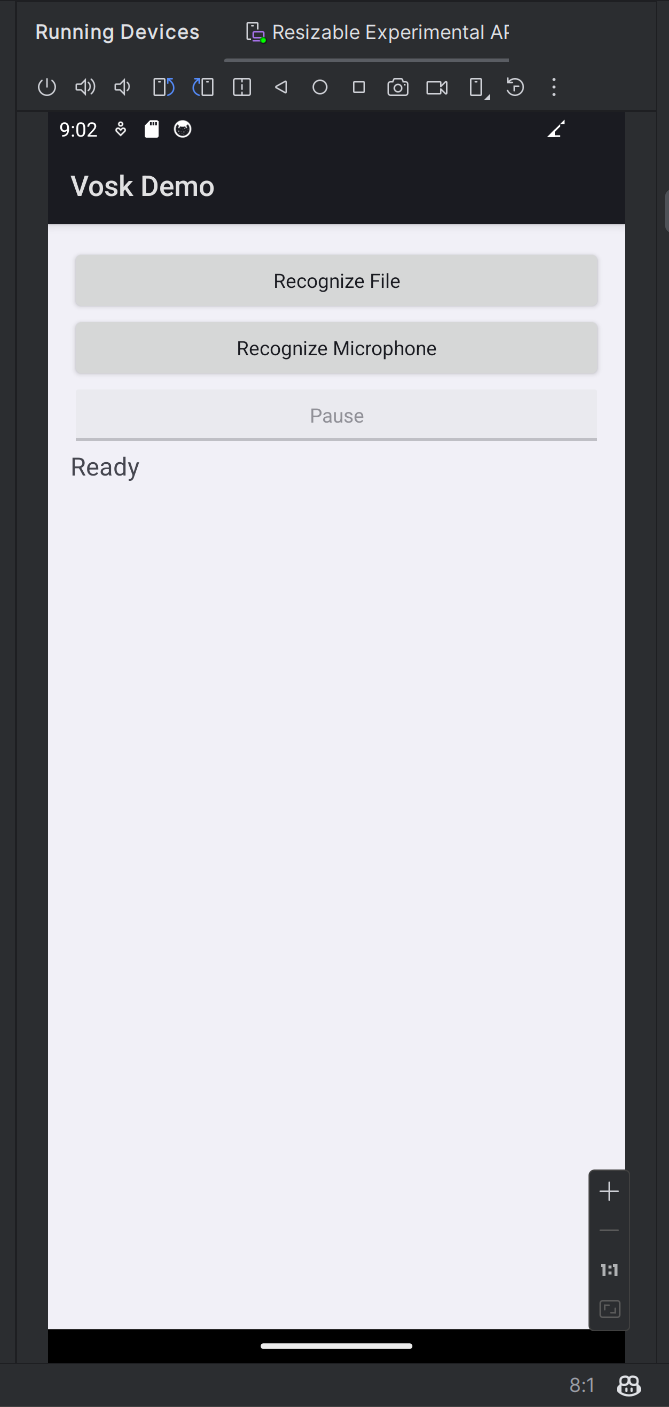
\includegraphics[scale=0.5]{Vosk_UI.png}
  \caption{UI van de Vosk demo applicatie}
\end{figure}

\subsection{Performantie}
De performantie van Vosk is afhankelijk van het gebruikte model. Vosk heeft per taal een groot en klein model. Het kleine model is ideaal voor bepaalde gelimiteerde toepassingen en heeft een grootte van ongeveer 50Mb. Het gebruikt ongeveer 300Mb aan geheugen tijdens de uitvoering, wat een ideaal model is voor mobiele toepassingen. Het grote model is ideaal voor toepassingen die een hogere accuraatheid vereisen. Dit model heeft een grootte van ongeveer 16Gb aan geheugen doordat het gebruik maakt van geavanceerde AI-algoritmes. Het nadeel van dit type model is dat de hardware krachtig genoeg moet zijn om de spraakherkenning uit te voeren. De ideale hardware voor dit model is een krachtige server, uitgerust met een Intel i7-processor of de nieuwste generatie AMD Ryzen-processoren. Het onderzoek richt zich op de talen Engels, Frans en Nederlands, waardoor er voor elke taal één specifiek spraakmodel is geselecteerd, in totaal dus drie spraakmodellen. Er is telkens gekozen voor het kleine model van Vosk, aangezien dit model ideaal is voor mobiele toepassingen. 
Volgende modellen worden gebruikt:

\begin{center}
  \begin{tabular}{ | l | l | l | p{5cm} |}
  \hline
  Modelnaam & Taalondersteuning & Grootte & Extra uitleg \\ \hline
  vosk-model-small-en-us-0.15 & US Engels & 40Mb & Klein model voor het Engels \\ \hline
  vosk-model-small-fr-0.22 & Frans & 41Mb & Klein model voor het Frans \\ \hline
  vosk-model-small-nl-0.22 & Nederlands & 39Mb & Klein model voor het Nederlands \\ \hline
  \end{tabular}
\end{center}



%%=============================================================================
%% Conclusie
%%=============================================================================

\chapter{Conclusie}%
\label{ch:conclusie}

% TODO: Trek een duidelijke conclusie, in de vorm van een antwoord op de
% onderzoeksvra(a)g(en). Wat was jouw bijdrage aan het onderzoeksdomein en
% hoe biedt dit meerwaarde aan het vakgebied/doelgroep? 
% Reflecteer kritisch over het resultaat. In Engelse teksten wordt deze sectie
% ``Discussion'' genoemd. Had je deze uitkomst verwacht? Zijn er zaken die nog
% niet duidelijk zijn?
% Heeft het onderzoek geleid tot nieuwe vragen die uitnodigen tot verder 
%onderzoek?

\lipsum[76-80]



%---------- Bijlagen -----------------------------------------------------------

\appendix

\chapter{Onderzoeksvoorstel}

Het onderwerp van deze bachelorproef is gebaseerd op een onderzoeksvoorstel dat vooraf werd beoordeeld door de promotor. Dat voorstel is opgenomen in deze bijlage.

%% TODO: 
%\section*{Samenvatting}

% Kopieer en plak hier de samenvatting (abstract) van je onderzoeksvoorstel.

% Verwijzing naar het bestand met de inhoud van het onderzoeksvoorstel
%---------- Inleiding ---------------------------------------------------------

\section{Introductie}%
\label{sec:introductie}
% Waarover zal je bachelorproef gaan? Introduceer het thema en zorg dat volgende zaken zeker duidelijk aanwezig zijn:

% \begin{itemize}
%   \item kaderen thema
%   \item de doelgroep
%   \item de probleemstelling en (centrale) onderzoeksvraag
%   \item de onderzoeksdoelstelling
% \end{itemize}

% Denk er aan: een typische bachelorproef is \textit{toegepast onderzoek}, wat betekent dat je start vanuit een concrete probleemsituatie in bedrijfscontext, een \textbf{casus}. Het is belangrijk om je onderwerp goed af te bakenen: je gaat voor die \textit{ene specifieke probleemsituatie} op zoek naar een goede oplossing, op basis van de huidige kennis in het vakgebied.

% De doelgroep moet ook concreet en duidelijk zijn, dus geen algemene of vaag gedefinieerde groepen zoals \emph{bedrijven}, \emph{developers}, \emph{Vlamingen}, enz. Je richt je in elk geval op it-professionals, een bachelorproef is geen populariserende tekst. Eén specifiek bedrijf (die te maken hebben met een concrete probleemsituatie) is dus beter dan \emph{bedrijven} in het algemeen.

% Formuleer duidelijk de onderzoeksvraag! De begeleiders lezen nog steeds te veel voorstellen waarin we geen onderzoeksvraag terugvinden.

% Schrijf ook iets over de doelstelling. Wat zie je als het concrete eindresultaat van je onderzoek, naast de uitgeschreven scriptie? Is het een proof-of-concept, een rapport met aanbevelingen, \ldots Met welk eindresultaat kan je je bachelorproef als een succes beschouwen?

%---------- Stand van zaken ---------------------------------------------------
De aanleiding voor de onderzoeksvraag ontstond vanuit het Mobile, Web en IoT-team van Delaware Consulting, dat graag onderzoek wilde doen naar de mogelijkheden van geïntegreerde spraaktechnologie. Dit is een technologie die spraakherkenning mogelijk maakt op apparaten met beperkte middelen, zoals bij afwezigheid van een internetverbinding. Met dit onderzoek wil Delaware Consulting een beter beeld krijgen van de mogelijkheden en beperkingen van geïntegreerde spraaktechnologie met als uiteindelijk \\doel dat het bedrijf in de toekomst een betere en efficiëntere service kan bieden aan zijn klanten.

Spraaktechnologie is de laatste jaren sterk geëvolueerd door de opkomst van AI en machine learning. Het is een actueel onderwerp dat veel aandacht krijgt in de media. Deze technologie kan een meerwaarde bieden voor specifieke applicaties in verschillende sectoren. Voordat deze technologie toegepast wordt, moet er eerst onderzocht worden welke spraakmodellen er bestaan en hoe die presteren onder verschillende omstandigheden. Aan de hand van deze probleemstelling is de onderzoeksvraag ``Wat zijn de mogelijkheden en beperkingen bij het implementeren van geïntegreerde spraaktechnologie in uitdagende omgevingsfactoren?'' ontstaan.

Het uiteindelijke resultaat van dit onderzoek is een proof-of-concept. Met behulp van de gekozen geïntegreerde spraakherkenningstechnologie uit de literatuurstudie wordt een applicatie ontwikkeld waarmee een takenlijst kan worden beheerd door middel van spraakherkenning. Hier komt zowel tekst-naar-spraak als spraak-naar-\\tekst aan bod. Met deze applicatie kan er dan een conclusie worden getrokken over de effectiviteit van deze spraakmodellen en hoe goed deze presteren in de realiteit. 



\section{Literatuurstudie}%
\label{sec:literatuurstudie}

Door de opkomst van artificiële intelligentie en machine learning is spraakherkenningstechnologie de laatste jaren sterk geëvolueerd. Spraakherkenning is een technologische mogelijkheid waarmee een softwareprogramma in staat is om gesproken menselijke taal om te zetten in geschreven tekst en omgekeerd. Het maakt het mogelijk om apparaten handsfree te bedienen en input automatisch te gaan vertalen. Om deze technologie te kunnen toepassen, moet er een microfoon aanwezig zijn op het apparaat om de trillingen van een stem om te zetten in een elektrisch signaal. Vervolgens wordt dit signaal omgezet in een digitaal signaal dat door een spraakherkenningsprogramma kan geanalyseerd worden.\autocite{Zwass2022}

Er zijn heel wat voordelen bij het gebruik van spraakherkenningstechnologie. Het is een snellere manier om tekst in te voeren dan bij het gebruik van een toetsenbord. Het is ook een handige tool voor mensen die problemen hebben met spreken of schrijven doordat deze spraakmodellen in staat zijn om van tekst-naar-spraak als van spraak-naar-tekst te gaan. Er zijn ook enkele nadelen aan verbonden. Zo is het niet altijd even nauwkeurig en kan het soms moeilijk zijn om de juiste woorden te herkennen. In het huidig stadium van de technologie is er controle nodig voor het corrigeren van fouten. \autocite{RingCentral2021}

Spraakherkenningsystemen hebben echter \\enkele uitdagingen. Het moeilijkste aspect is de taaldekking voor de spraakmodellen doordat er heel veel verschillende talen bestaan en elke taal zijn eigen accenten en dialecten heeft. Een ander belangrijk spraakherkenningsprobleem is achtergrondlawaai doordat dit mee wordt opgenomen door de microfoon. Dit kan de spraakherkenning verstoren en de nauwkeurigheid van het spraakmodel verminderen. Bij het gebruik van spraakherkenningstechnologie is het belangrijk om rekening te houden met de privacy van de gebruiker, wat een essentieel aandachtspunt is tijdens de implementatie. \autocite{Singh2022}

De bekendste spraakherkenningstechno-\\logieën zijn: Microsoft Azure Cognitive Speech, Google Cloud Speech-to-Text, Amazon Transcribe, IBM Watson, Mozilla DeepSpeech en Whisper.ai. Deze spraakmodellen zijn bekend omdat ze afkomstig zijn van grote bedrijven met voldoende middelen om deze technologieën te ontwikkelen. Een aantal van deze spraakmodellen zijn cloud-gebaseerd en hebben dus een internetverbinding nodig om te kunnen werken. Bepaalde spraakmodellen bieden ook functionaliteiten voor offline gebruik door middel van een SDK die op het apparaat geïnstalleerd kan worden. Elk model heeft zijn eigen voor- en nadelen, waardoor je ze kunt gaan vergelijken. De keuze van het model is afhankelijk van de behoeften van het project. \autocite{Fox2023}

Microsoft Azure Cognitive Speech is een platform dat zich richt op de ontwikkeling van spraakherkenningstechnologie. De Text-to-Speech en Speech-to-Text modellen zijn onderdelen van dit platform waarbij beide modellen een cloud-\\gebaseerde API hebben die een internetverbinding nodig heeft om te kunnen werken. Via het installeren van een SDK is het mogelijk om apparaten offline te laten werken met deze modellen. Op dit platform zijn ook andere spraakmodellen aanwezig zoals Translation en Speaker Recognition. \autocite{Depypere2023}

Google Cloud Speech-to-Text is een spraakherkenningstechnologie die ontwikkeld is door Google. Het ondersteunt meer dan 120 talen en dialecten. Voor de implementatie van deze technologie is een cloud-gebaseerde API vereist die een internetverbinding nodig heeft. Een nadeel is dat dit model niet zonder internetverbinding kan werken. Deze technologie is één van de meest nauwkeurige spraakmodellen die er bestaan op dit moment. Het biedt heel wat features aan zoals het mogelijk maken om een eigen custom spraakmodel te trainen of het herkennen van verschillende sprekers. \autocite{Wang2021}

Amazon Transcribe maakt het mogelijk om spraak om te zetten naar tekst en omgekeerd. Het model biedt voor meerdere talen ondersteuning aan waarbij het mogelijk is om realtime transcriptie toe te passen. Het model is cloud-\\gebaseerd en heeft dus een internetverbinding nodig om te kunnen werken. Dit model heeft een hoge nauwkeurigheid en is in staat om achtergrondlawaai te filteren. \autocite{Kumbhar2023}

Mozilla DeepSpeech is een open-source spraakherkenningstechnologie die is ontwikkeld door Mozilla, de organisatie achter de welbekende \\browser Firefox. Dit model staat bekend om zijn offline functionaliteit en is volledig gratis. Het model moet wel getraind worden om een goede nauwkeurigheid te hebben. Het model is nog in ontwikkeling, dus het is niet zo nauwkeurig en snel als de voorgaande modellen. Het ondersteunt enkel spraak naar tekst en niet omgekeerd. \autocite{Tang2022}

Whisper.ai is een spraakherkenningstechnologie dat ontwikkeld is door het welgekende OpenAI. Dit bedrijf is bekend door zijn onderzoek naar artificiële intelligentie. De technologie is open-source en kan volledig offline werken. Het heeft verschillende modellen waarbij je kunt kiezen tussen modellen met een hogere nauwkeurigheid of een snellere verwerkingstijd door de grootte van het model aan te passen. Het model biedt ondersteuning aan voor meerdere talen die een eigen score hebben gekregen op basis van de nauwkeurigheid. Deze score is gebaseerd op de WER (Word Error Rate) die aangeeft hoeveel woorden er fout zijn herkend. \autocite{OpenAI2023}

Om de spraakherkenningsmodellen te vergelijken, zijn er verschillende methoden beschikbaar om dit te doen. Woordfoutpercentage (WER) is bekende methode die de fouten die gemaakt worden bij woorden, tussen de input en de output meet en gaat weergeven aan de hand van een percentage. De snelheid van een model kan ook gemeten worden door de verwerkingstijd te meten bij het uitvoeren van dezelfde dataset.\\ \autocite{OConnor2023}


% Hier beschrijf je de \emph{state-of-the-art} rondom je gekozen onderzoeksdomein, d.w.z.\ een inleidende, doorlopende tekst over het onderzoeksdomein van je bachelorproef. Je steunt daarbij heel sterk op de professionele \emph{vakliteratuur}, en niet zozeer op populariserende teksten voor een breed publiek. Wat is de huidige stand van zaken in dit domein, en wat zijn nog eventuele open vragen (die misschien de aanleiding waren tot je onderzoeksvraag!)?

% Je mag de titel van deze sectie ook aanpassen (literatuurstudie, stand van zaken, enz.). Zijn er al gelijkaardige onderzoeken gevoerd? Wat concluderen ze? Wat is het verschil met jouw onderzoek?

% Verwijs bij elke introductie van een term of bewering over het domein naar de vakliteratuur, bijvoorbeeld~\autocite{Hykes2013}! Denk zeker goed na welke werken je refereert en waarom.

% Draag zorg voor correcte literatuurverwijzingen! Een bronvermelding hoort thuis \emph{binnen} de zin waar je je op die bron baseert, dus niet er buiten! Maak meteen een verwijzing als je gebruik maakt van een bron. Doe dit dus \emph{niet} aan het einde van een lange paragraaf. Baseer nooit teveel aansluitende tekst op eenzelfde bron.

% Als je informatie over bronnen verzamelt in JabRef, zorg er dan voor dat alle nodige info aanwezig is om de bron terug te vinden (zoals uitvoerig besproken in de lessen Research Methods).

% % Voor literatuurverwijzingen zijn er twee belangrijke commando's:
% % \autocite{KEY} => (Auteur, jaartal) Gebruik dit als de naam van de auteur
% %   geen onderdeel is van de zin.
% % \textcite{KEY} => Auteur (jaartal)  Gebruik dit als de auteursnaam wel een
% %   functie heeft in de zin (bv. ``Uit onderzoek door Doll & Hill (1954) bleek
% %   ...'')

% Je mag deze sectie nog verder onderverdelen in subsecties als dit de structuur van de tekst kan verduidelijken.



%---------- Methodologie ------------------------------------------------------
\section{Methodologie}%
\label{sec:methodologie}

Het onderzoek is opgedeeld in vijf opeenvolgende fases. In de eerste fase wordt informatie verzameld over de verschillende spraakmodellen en hun werking, met focus op modellen die met beperkte middelen kunnen werken. Deze informatie zal worden verzameld door een grondige studie van vakliteratuur. De geschatte duurtijd van deze fase bedraagt een tweetal weken. 

In de daaropvolgende fase zal een vergelijkende studie worden uitgevoerd waarbij de verschillende spraakmodellen worden vergeleken op basis van hun prestaties door met deze modellen te experimenten. Hierbij wordt gekeken naar hun nauwkeurigheid en prestaties in verschillende omgevingsfactoren voor de talen Nederlands, Frans en Engels. Op basis van deze vergelijking wordt er een spraakmodel gekozen dat zal worden gebruikt voor de proof-of-concept. De geschatte duurtijd van deze fase bedraagt een drietal weken.

In de derde fase wordt een applicatieontwerp gecreëerd, waarbij wireframes worden gebruikt om de gebruikersinterface visueel weer te geven. Deze fase zal naar verwachting ongeveer 1 week duren.

In de vierde fase wordt de implementatie van de applicatie uitgevoerd. Hierbij wordt de gekozen spraaktechnologie geïntegreerd in de applicatie. De geschatte duurtijd van deze fase bedraagt een tweetal weken.

In de afsluitende fase van het onderzoek wordt de geïmplementeerde proof-of-concept \\beoordeeld en geanalyseerd in de realiteit. Het doel is om vast te stellen in hoeverre de gestelde doelstellingen zijn behaald en om inzichten te verkrijgen voor eventuele verbeteringen of aanpassingen. Hierbij wordt een evaluatierapport ontwikkeld waarin de verzamelde analyse van de resultaten wordt samengevat en conclusies worden getrokken met betrekking tot de bruikbaarheid en effectiviteit van het toegepaste spraakmodel. De geschatte duurtijd van deze fase bedraagt een tweetal weken.


% Hier beschrijf je hoe je van plan bent het onderzoek te voeren. Welke onderzoekstechniek ga je toepassen om elk van je onderzoeksvragen te beantwoorden? Gebruik je hiervoor literatuurstudie, interviews met belanghebbenden (bv.~voor requirements-analyse), experimenten, simulaties, vergelijkende studie, risico-analyse, PoC, \ldots?

% Valt je onderwerp onder één van de typische soorten bachelorproeven die besproken zijn in de lessen Research Methods (bv.\ vergelijkende studie of risico-analyse)? Zorg er dan ook voor dat we duidelijk de verschillende stappen terug vinden die we verwachten in dit soort onderzoek!

% Vermijd onderzoekstechnieken die geen objectieve, meetbare resultaten kunnen opleveren. Enquêtes, bijvoorbeeld, zijn voor een bachelorproef informatica meestal \textbf{niet geschikt}. De antwoorden zijn eerder meningen dan feiten en in de praktijk blijkt het ook bijzonder moeilijk om voldoende respondenten te vinden. Studenten die een enquête willen voeren, hebben meestal ook geen goede definitie van de populatie, waardoor ook niet kan aangetoond worden dat eventuele resultaten representatief zijn.

% Uit dit onderdeel moet duidelijk naar voor komen dat je bachelorproef ook technisch voldoen\-de diepgang zal bevatten. Het zou niet kloppen als een bachelorproef informatica ook door bv.\ een student marketing zou kunnen uitgevoerd worden.

% Je beschrijft ook al welke tools (hardware, software, diensten, \ldots) je denkt hiervoor te gebruiken of te ontwikkelen.

% Probeer ook een tijdschatting te maken. Hoe lang zal je met elke fase van je onderzoek bezig zijn en wat zijn de concrete \emph{deliverables} in elke fase?

%---------- Verwachte resultaten ----------------------------------------------
\section{Verwacht resultaat, conclusie}%
\label{sec:verwachte_resultaten}

% Hier beschrijf je welke resultaten je verwacht. Als je metingen en simulaties uitvoert, kan je hier al mock-ups maken van de grafieken samen met de verwachte conclusies. Benoem zeker al je assen en de onderdelen van de grafiek die je gaat gebruiken. Dit zorgt ervoor dat je concreet weet welk soort data je moet verzamelen en hoe je die moet meten.

% Wat heeft de doelgroep van je onderzoek aan het resultaat? Op welke manier zorgt jouw bachelorproef voor een meerwaarde?

% Hier beschrijf je wat je verwacht uit je onderzoek, met de motivatie waarom. Het is \textbf{niet} erg indien uit je onderzoek andere resultaten en conclusies vloeien dan dat je hier beschrijft: het is dan juist interessant om te onderzoeken waarom jouw hypothesen niet overeenkomen met de resultaten.

Er wordt verwacht dat de geïmplementeerde proof-of-concept een applicatie is waarmee tijd kan worden bespaard bij het beheren van een takenlijst. Personen met visuele of motorische beperkingen, evenals degenen die moeite hebben met typen of schrijven zullen baat hebben bij deze oplossing. 

Op basis van het evaluatierapport zouden de uitdagingen in kaart moeten worden gebracht die zich voordoen bij het gebruik van deze geïntegreerde spraaktechnologie. Er wordt verwacht dat de uitdagingen vooral zullen liggen bij de taalkeuze en de omgevingsfactoren.

De ontwikkeling van het proof-of-concept kan bijdragen aan het begrijpen en uitbreiden van spraaktechnologie. In de toekomst zal spraaktechnologie met geavanceerde AI en machine learning verder worden verbeterd, wat kan leiden tot betere prestaties en meer toegevoegde waarde in andere sectoren.


%%---------- Andere bijlagen --------------------------------------------------
% TODO: Voeg hier eventuele andere bijlagen toe. Bv. als je deze BP voor de
% tweede keer indient, een overzicht van de verbeteringen t.o.v. het origineel.
%\input{...}

%%---------- Backmatter, referentielijst ---------------------------------------

\backmatter{}

\setlength\bibitemsep{2pt} %% Add Some space between the bibliograpy entries
\printbibliography[heading=bibintoc]

\end{document}